\documentclass{article}
\usepackage[utf8]{inputenc}
\usepackage[T1]{fontenc}
\usepackage[ngerman]{babel}
\usepackage[
    left = \glqq{},% 
    right = \grqq{},% 
    leftsub = \glq{},% 
    rightsub = \grq{} %
]{dirtytalk}
\usepackage{graphicx}
\graphicspath{ {./assets/} }

\title{SEN}
\author{Felix Hofinger}
\date{October 2022}

\setcounter{secnumdepth}{4}
\setcounter{tocdepth}{4}

\begin{document}

\maketitle
\newpage
\tableofcontents
\newpage

\section{Datenabfrage}

\begin{verbatim}
    SELECT [DISTINCT] 
        {* | Attributliste | mathematische Ausdrücke } Bezeichner
    FROM Tabelle1 Bezeichner1, Tabelle 2 Bezeichner2, ...
    [WHERE BEDINGUNG]
    [GROUP BY Attributliste] [HAVING Bedingung]
    [ORDER BY Attributliste] [ASC | DESC]
\end{verbatim}

\subsection{Einfache Abfrage}

\begin{verbatim}
    SELECT *
    FROM Kursthemen
\end{verbatim}

\begin{table}[!htbp]
  \center
  \begin{tabular}{c|c}
    TNr & Themengebiet                \\
    \hline
    1   & Sicherheit und Umweltschutz \\
    2   & ...
  \end{tabular}
  \label{tab:select:1}
  \caption{Beispiel Ergebnis}
\end{table}

\hrule

\begin{verbatim}
    SELECT PNr, Name, Vorname, 
      (Lohnstufe - 1) * 10000 + 60000 Salary
    FROM Personen
\end{verbatim}

\begin{table}[!htbp]
  \center
  \begin{tabular}{c|c|c|c}
    PNr    & Name    & Vorname & Salary \\
    \hline
    100001 & Steffen & Felix   & 100000 \\
    ...    &         &         &
  \end{tabular}
  \label{tab:select:2}
  \caption{Beispiel Ergebnis}
\end{table}

\subsection{Bedingung}

\begin{verbatim}
    SELECT PNr, Name, Vorname
    FROM Personen
    WHERE FNr = 1
\end{verbatim}

\newpage
\subsection{Datensätze sortieren}

\begin{verbatim}
    SELECT *
    FROM Funktionen
    ORDER BY Funktion
\end{verbatim}

\begin{table}[!htbp]
  \center
  \begin{tabular}{c|c}
    FNr & Funktion       \\
    \hline
    4   & Bereichsleiter \\
    ...
  \end{tabular}
  \label{tab:order:1}
  \caption{Beispiel Ergebnis}
\end{table}

\subsection{Datensätze gruppieren}

% TODO: FIX THIS

\begin{table}[!htbp]
  \center
  \begin{tabular}{ccccc}
    PNr & VN & KN & FNr & Salary \\
    \hline
    1   &    &    & 3   &        \\
    2   &    &    & 3   &        \\
    3   &    &    & 4   &        \\
    4   &    &    & 5   &        \\
    5   &    &    & 4   &        \\
    6   &    &    & 4   &        \\
    7   &    &    & 4   &        \\
    8   &    &    & 3   &        \\
  \end{tabular}
  \quad
  =>
  \quad
  \begin{tabular}{ccccc}
    FNr & \\
    \hline
    3   & \\
    4   & \\
    5   & \\
  \end{tabular}
  \label{tab:group:1}
  \caption{Beispiel: \protect\say{GROUP BY}}
\end{table}

\begin{verbatim}
    SELECT FNr, COUNT(FNr) Anzahl, 
      AVG(Lohnstufe - 1) * 10000 + 60000 Salary
    FROM Personen
    GROUP BY FNr
    ORDER BY FNr DESC
\end{verbatim}

\vspace{0.5em}
\begin{flushleft}
  In Verbindung mit dem Schlüsselwort \say{GROUP BY} gibt es noch
  das Schlüsselwort \say{HAVING} welches das definieren von Gruppenbedingungen ermöglicht.
  Im Gegensatz zu \say{WHERE} werden die mit \say{HAVING} angegebenen Bedingungen nicht
  auf einzelne Datensätze, sondern auf Datensatzgruppen angewendet.
\end{flushleft}

\newpage
\subsection{Verschachtelte Abfragen}

\begin{verbatim}
    SELECT KNr, Kursbezeichnung
    FROM Kurse
    WHERE KNr IN (
      SELECT KNr
      FROM Kursbesuche
      WHERE PNr = (
        SELECT PNr
        FROM Personen
        WHERE Name = 'Steffen'
        AND Vorname = 'Felix'
      )
    )
    ORDER BY Kursbezeichnung
\end{verbatim}

\vspace{0.5em}
\hrule
\vspace{0.6em}

\begin{verbatim}
  SELECT FNr, Name, Vorname, Lohnstufe
  FROM Personen
  WHERE (FNr, Lohnstufe) IN (
    SELECT FNr, MAX(Lohnstufe)
    FROM Personen
    GROUP BY FNr
  )
  ORDER BY FNr DESC, Name ASC
\end{verbatim}

\subsection{Tabellen verknüpfen (Joining)}

\begin{table}[!htbp]
  \center
  \begin{tabular}{c|c|c}
    A           & B      & C      \\
    \hline
    \textrm{I}  & $\sim$ & $\sim$ \\
    \textrm{II} & $\sim$ & $\sim$ \\
  \end{tabular}
  \quad
  X
  \quad
  \begin{tabular}{c|c|c}
    D        & E      & F      \\
    \hline
    $\alpha$ & $\sim$ & $\sim$ \\
    $\beta$  & $\sim$ & $\sim$ \\
  \end{tabular}

  \vspace{1.2em}
  \begin{tabular}{c|c|c|c|c|c}
    A           & B      & C      & D        & E      & F      \\
    \hline
    \textrm{I}  & $\sim$ & $\sim$ & $\alpha$ & $\sim$ & $\sim$ \\
    \textrm{I}  & $\sim$ & $\sim$ & $\beta$  & $\sim$ & $\sim$ \\
    \textrm{II} & $\sim$ & $\sim$ & $\alpha$ & $\sim$ & $\sim$ \\
    \textrm{II} & $\sim$ & $\sim$ & $\beta$  & $\sim$ & $\sim$ \\
  \end{tabular}
  \quad
  SELECT * FROM Funktionen, Personen
  \label{tab:join:1}
  \caption{Beispiel: \protect\say{CROSS JOIN}}
\end{table}

\begin{table}[!htbp]
  \center
  \begin{tabular}{c|c|c}
    A            & B      & $C^{'}$  \\
    \hline
    \textrm{I}   & $\sim$ & $\alpha$ \\
    \textrm{II}  & $\sim$ & $\alpha$ \\
    \textrm{III} & $\sim$ & $\beta$  \\
  \end{tabular}
  \quad
  X
  \quad
  \begin{tabular}{c|c|c}
    $C^{''}$ & D      & E      \\
    \hline
    $\alpha$ & $\sim$ & $\sim$ \\
    $\beta$  & $\sim$ & $\sim$ \\
  \end{tabular}

  \vspace{1.2em}
  \begin{tabular}{c|c|c|c|c|c}
    A            & B      & $C^{'}$  & $C^{''}$ & D      & E      \\
    \hline
    \textrm{I}   & $\sim$ & $\alpha$ & $\alpha$ & $\sim$ & $\sim$ \\
    \textrm{II}  & $\sim$ & $\alpha$ & $\alpha$ & $\sim$ & $\sim$ \\
    \textrm{III} & $\sim$ & $\beta$  & $\beta$  & $\sim$ & $\sim$ \\
  \end{tabular}
  \quad
  \begin{tabular}{l}
    SELECT *                  \\
    FROM Funktionen, Personen \\
    WHERE Funktionen.FNr = Personen.FNr
  \end{tabular}
  \label{tab:join:2}
  \caption{Beispiel: \protect\say{INNER JOIN}}
\end{table}

\newpage
\subsubsection{Die 4 Join-Arten}

\begin{table}[!htbp]
  \center
  \begin{tabular}{c|c|c}
    A            & B      & C  \\
    \hline
    \textrm{I}   & $\sim$ & 1  \\
    \textrm{II}  & $\sim$ & 2  \\
    \textrm{III} & $\sim$ & 2  \\
    \textrm{IV}  & $\sim$ & 99 \\
  \end{tabular}
  \quad
  X
  \quad
  \begin{tabular}{c|c|c}
    D & E  & F      \\
    \hline
    a & 1  & $\sim$ \\
    b & 2  & $\sim$ \\
    d & 55 & $\sim$ \\
  \end{tabular}
  \label{tab:joins:1}
  \caption{Beispiel Tabellen für die 4 Join-Arten}
\end{table}

\begin{table}[!htbp]
  \center
  \underline{inner join:}
  \quad
  \raisebox{-15pt}{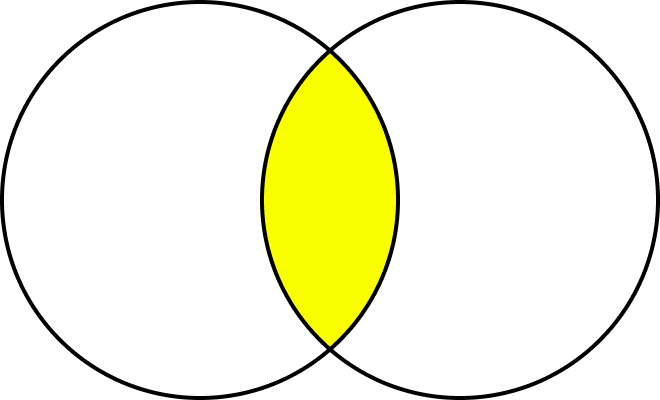
\includegraphics[scale=0.35]{/1/6/inner_join}}
  \quad
  \begin{tabular}{c|c|c|c|c|c}
    A            & B      & C & D & E & F      \\
    \hline
    \textrm{I}   & $\sim$ & 1 & a & 1 & $\sim$ \\
    \textrm{II}  & $\sim$ & 2 & b & 2 & $\sim$ \\
    \textrm{III} & $\sim$ & 2 & b & 2 & $\sim$ \\
  \end{tabular}
  \label{tab:joins:2}
\end{table}

\begin{table}[!htbp]
  \center
  \underline{left join:}
  \quad
  \raisebox{-15pt}{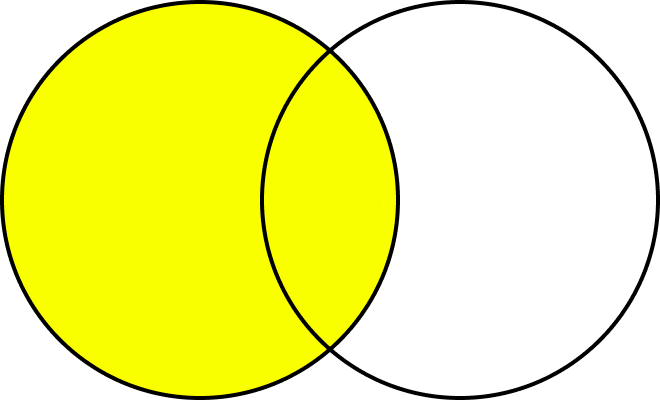
\includegraphics[scale=0.35]{/1/6/left_join}}
  \quad
  \begin{tabular}{c|c|c|c|c|c}
    A            & B      & C  & D    & E    & F      \\
    \hline
    \textrm{I}   & $\sim$ & 1  & a    & 1    & $\sim$ \\
    \textrm{II}  & $\sim$ & 2  & b    & 2    & $\sim$ \\
    \textrm{III} & $\sim$ & 2  & b    & 2    & $\sim$ \\
    \textrm{IV}  & $\sim$ & 99 & NULL & NULL & NULL   \\
  \end{tabular}
  \label{tab:joins:3}
\end{table}

\begin{table}[!htbp]
  \center
  \underline{right join:}
  \quad
  \raisebox{-15pt}{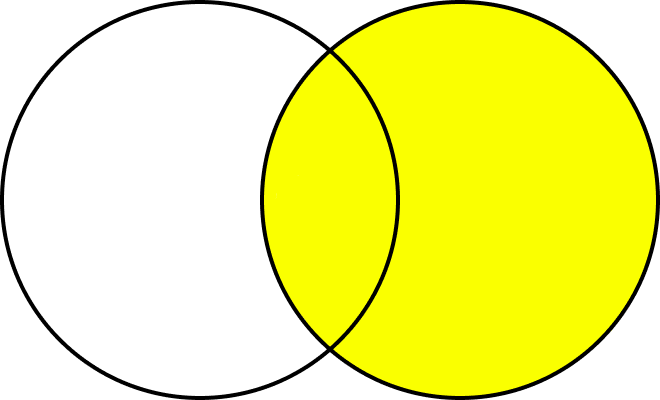
\includegraphics[scale=0.35]{/1/6/right_join}}
  \quad
  \begin{tabular}{c|c|c|c|c|c}
    A            & B      & C    & D & E  & F      \\
    \hline
    \textrm{I}   & $\sim$ & 1    & a & 1  & $\sim$ \\
    \textrm{II}  & $\sim$ & 2    & b & 2  & $\sim$ \\
    \textrm{III} & $\sim$ & 2    & b & 2  & $\sim$ \\
    NULL         & NULL   & NULL & d & 55 & $\sim$ \\
  \end{tabular}
  \label{tab:joins:4}
\end{table}

\underline{cross join:}
\quad
Jedes Tupel mit jedem

\end{document}
